\chapter{Linear Optics from Closed Orbits Method}\label{chap:loco}
\gls{loco}, is a model-dependent algorithm whose the main objective is to calibrate the accelerator model in order to reproduce the measured orbit response matrix in the real machine. Once this correspondence is achieved, it is considered that the calibrated model is a representation of the real machine in terms of the linear response of the magnetic lattice. Therefore, one can access the information from the real accelerator by analysing the model. The principal information that is studied in this process is related to the linear optics functions (betatron and dispersion functions), allowing for disturbances detection and, more importantly, to determine the corrections, pushing the measured linear optics to the nominal values.

This method has been applied to several synchrotron light sources over the years and has been proven to be efficient both to detect optics perturbations and to correct the machine linear optics~\cite{safranek1997, icfa_laurent, icfa_australia}. Besides that, with the realization of 4\ts{th} generation light sources, which use innovative and very compact magnetic lattices and optics, some details and subtleties of LOCO should be revisited to successfully apply the method in modern machines such as Sirius storage ring. This chapter is dedicated to present LOCO method and to discuss the aforementioned details.
\section{Orbit Response Matrix Analysis}\label{sec:orm_analysis}
If a $j$-th dipolar corrector strength is locally varied by the amount $\Delta \theta_j$, the electron closed orbit is distorted. The horizontal and vertical distortions ($\Delta x$ and $\Delta y$) can be measured by the~\gls{bpm}s. With the distortions measured by the $i$-th~\gls{bpm}, the following quantities can be calculated in this process:
\begin{align}
    M^{uv}_{ij} &= \dfrac{\Delta u_i}{\Delta \theta_j^v}.
\end{align}

If the corrector magnet is horizontal, $v=x$ and if it is vertical, $v=y$. For each corrector varied, one can measure the corresponding positions variations given by every~\gls{bpm}, horizontally $u=x$ and vertically $u=y$. These values can be cast in an array $\mathbf{M}$, called~\gls{orm}. Usually the element ordering in this matrix is the following:
\begin{equation}
    \mathbf{M} = \begin{bmatrix}
    \mathbf{M}^{xx} & \mathbf{M}^{xy} \\
    \mathbf{M}^{yx} & \mathbf{M}^{yy} 
\end{bmatrix}.
\end{equation}

The sub-matrices $\mathbf{M}^{xx}$ and $\mathbf{M}^{yy}$ in the diagonal blocks are the elements with larger values in the~\gls{orm}. In a magnetic lattice with zero transverse coupling (such as the nominal magnetic lattice for Sirius storage ring) the sub-matrices $\mathbf{M}^{xy}$ and $\mathbf{M}^{yx}$ in the off-diagonal blocks are zero. The order of magnitude of the elements in off-diagonal blocks compared to the diagonal blocks is smaller by the same order of magnitude of the transverse coupling, typically a few percent without corrections.

For the uncoupled case, it is possible to obtain an analytical expression for the~\gls{orm} elements in the diagonal blocks. In Eq.~\eqref{eq:orbit_distortion}, the orbit distortion in the presence of a given dipolar kick distribution $\theta_u(s)$ was shown. For the special case that the kick distribution is discrete, localized in the dipolar correctors positions $s_j$, with values $\Delta \theta^{u}_{j}$, Eq.~\eqref{eq:orbit_distortion} is rewritten in the form:
\begin{equation}
    \Delta u(s_i) = \sum_{j} \dfrac{\sqrt{\beta_{u}(s_i)\beta_{u_j}(s_j)}}{2\sin\left(\pi\nu_{u}\right)} \Delta \theta^{u}_j \cos\left( |\varphi_{u}(s_i) - \varphi_{u}(s_j)| - \pi\nu_{u} \right).
    \label{eq:discrete_orbit_distortion}
\end{equation}

The orbit distortions $\Delta u(s_i)$ are also measured in discrete and localized positions $s_i$, where the~\gls{bpm}s are installed. The above equation can be cast in the form $\Delta u_i = \sum_{j} M_{ij}^{uu} \Delta \theta_{j}^{u}$, therefore the~\gls{orm} elements can be recognized as:
\begin{align}
M_{ij}^{uu} = \dfrac{\sqrt{\beta_{u}(s_i)\beta_{u}(s_j)}}{2\sin\left(\pi\nu_{u}\right)}\cos\left( |\varphi_{u}(s_i) - \varphi_{u}(s_j)| - \pi\nu_{u} \right).
\label{eq:matrix_elements}
\end{align}

Note that the~\gls{orm} elements contain information about the local betatron function in the~\gls{bpm}s and correctors positions. It also encodes the relative betatron phase advance between each pair of BPM and steering magnet and the~\gls{orm} also depends on the betatron tune, a global parameter. 

Following the sorting used in the~\gls{orm}, the orbit distortions and the dipolar kick variations can be arranged in vectors
\begin{align*}
    \Delta \vec{u} &= \left(\Delta x_1, \ldots, \Delta x_{\mathrm{N}_{\mathrm{BPM}}}, \Delta y_1, \ldots, \Delta y_{\mathrm{N}_{\mathrm{BPM}}}\right), \\
    \Delta \vec{\theta} &= \left(\Delta \theta_1^x, \ldots, \Delta \theta_{\mathrm{N}_{\mathrm{CH}}}^x, \Delta \theta_1^y, \ldots, \Delta \theta_{\mathrm{N}_{\mathrm{CV}}}^y\right).
\end{align*}

$\mathrm{N}_{\mathrm{BPM}}$ is the number of~\gls{bpm}s, $\mathrm{N}_{\mathrm{CH}}$ is the number of horizontal correctors (CH) and $\mathrm{N}_{\mathrm{CV}}$ is the number of vertical correctors (CV). The orbit correction system for Sirius storage ring has $\mathrm{N}_{\mathrm{BPM}} = 160$, $\mathrm{N}_{\mathrm{CH}} = 120$ and $\mathrm{N}_{\mathrm{CV}} = 160$.  In this vectorial form, Eq.~\eqref{eq:discrete_orbit_distortion} is $\Delta \vec{u} = \mathbf{M} \Delta \vec{\theta}$, so the~\gls{orm} has dimension $2 \mathrm{N}_{\mathrm{BPM}} \times \left(\mathrm{N}_{\mathrm{CH}} + \mathrm{N}_{\mathrm{CV}}\right)$. 

Suppose that the~\gls{bpm}s measure the orbit distortion $\vec{u}_{\mathrm{d}}$. With the dipolar correctors it is possible to produce an orbit variation that minimizes the 2-norm of the residual orbit. Minimizing $||\vec{u}_{\mathrm{d}} - \mathbf{M}\Delta \vec{\theta}||^2$ with respect to $\Delta\vec{\theta}$, one obtain that the required kicks variations are $\Delta \vec{\theta} = -\left(\mathbf{M}^{\mathsf{T}}\mathbf{M}\right)^{-1}\mathbf{M}^{\mathsf{T}}\vec{u}_{\mathrm{d}}$. Since the actual problem is non-linear, the corrections must be calculated and applied iteratively until convergence. 

The pseudo-inverse of $\mathbf{M}^{\mathsf{T}}\mathbf{M}$ may be obtained with the method of~\gls{svd} pseudo-inversion which is described in Appendix~\ref{appendix:svd}. Using this method and, depending on the number of fit parameters compared to the number of data points, it is also possible to minimize the correctors strengths required to minimize the figure of merit, in this case, the orbit distortion 2-norm.

% Generally, $2\mathrm{N}_{\mathrm{BPM}} \neq \mathrm{N}_{\mathrm{CH}} + \mathrm{N}_{\mathrm{CV}}$, then the~\gls{orm} is a rectangular matrix and $\mathbf{M}^{-1}$ is not an ordinary inverse. 
It is common to also include the~\gls{rf} frequency as a knob in the orbit correction system. This can be done by adding in the last column of the~\gls{orm} the orbit distortion vector produced by a variation in the RF frequency. From Eq.~\eqref{eq:delta_freq} and using $\Delta u_i = \eta_u(s_i) \delta$, we obtain:
\begin{equation}
    \dfrac{\Delta u_i}{ \Delta f_{\mathrm{rf}}} = - \dfrac{\eta_u(s_i)}{\alpha f_{\mathrm{rf}}}.
    \label{eq:rf_column}
\end{equation}

Adding this extra knob to the orbit correction system is very important to correct orbit length variations, which can be generated by thermal drifts of the storage ring tunnel, tidal effects, etc. It is important to observe that the~\gls{rf} signature in the orbit distortion is very different from the signature created by the correctors, since the first depends on the dispersion function and the latter on the betatron function.
% In this way, the correction calculations for the orbit distortions also provides a variation in the~\gls{rf} frequency (this is useful to correct variations in the orbit length, for example, produced thermal variations in the storage ring tunnel). It is important to observe that the~\gls{rf} signature in the orbit distortion is very different from the signature created by the correctors, since the first depends on the dispersion function and the latter on the betatron function.

The~\gls{orm} with the RF frequency column added is then a matrix with dimension $2 \mathrm{N}_{\mathrm{BPM}} \times \left(\mathrm{N}_{\mathrm{CH}} + \mathrm{N}_{\mathrm{CV}}+1\right)$. For the Sirius storage ring, the~\gls{orm} is a $320 \times 281$ matrix. Beyond the function of calculating the corrections for orbit distortions, the~\gls{orm} contains a lot of information about the uncoupled linear optics (betatron function, phase advance and horizontal dispersion function) and the coupled linear optics (betatron coupling and vertical dispersion function).~\gls{loco} method explores extensively the information contained in the~\gls{orm}.

% Based on the phase stability principle, for a fixed~\gls{rf} frequency, the orbit length is constant as well. On the other hand, one can notice that a dipolar kick located in a dispersive region produces a change in the orbit length given by $\Delta x = -\eta_x(s_j)\theta_j$, where $s_j$ is the corrector longitudinal position. To maintain the orbit length fixed the electron energy must change. From Eq.~\eqref{orbitlen}, the orbit length change for a given energy deviation is $\Delta L = \alpha L_0 \delta$, then to obtain $\Delta L + \Delta x = 0$, the corresponding energy shift is $\delta = \dfrac{\eta_x(s_j) \theta_j}{\alpha L_0}$. 

% If the~\gls{orm} numerical calculation is performed using only the transverse components, disregarding the energy loss and gain processes, the energy shifts due to the dipolar kicks are not included in the~\gls{orm} elements. The energy shift $\delta$ generates the orbit distortion given by $\Delta x_i = \eta_x(s_i)\delta$, therefore the elements of $\mathbf{M}^{xx}$ must be changed by~\cite{huang2019beam}:
% \begin{equation}
%     M_{ij}^{xx} \rightarrow M_{ij}^{xx} + \dfrac{\eta_x(s_i)\eta_x(s_j)}{\alpha L_0}.
% \end{equation}

% If the~\gls{orm} calculation includes the radiation loss and the energy gain by the~\gls{rf} cavity, the orbit length is fixed by the phase stability principle and the energy shifts contributions in the~\gls{orm} is automatically included\footnote{The numerical calculations performed with transverse coordinates are typically called 4D simulations and when it includes the transverse and longitudinal coordinates it is called 6D simulations.}.

% \begin{align}
%     u_i\left({\theta_j^u+\Delta\theta_j^u}\right) = u_i\left(\theta_j^u\right) + \dfrac{\partial u_i}{\partial \theta_j^u} \Delta \theta_j^u
% \end{align}

% \begin{equation}
%     M^{u u}_{ij} = \dfrac{\Delta u_i (+\Delta \theta_j^u/2) - \Delta u_i (-\Delta \theta_j^u/2)}{\Delta \theta_j^u}.
%     \label{medida}
% \end{equation}

% $M_{ij} = \dfrac{\partial u_i}{\partial \theta_j^u} + O(3)$.
\section{Minimization Problem}
To implement LOCO method, a storage ring model is required. In this model, it is possible to calculate the nominal~\gls{orm}. That can be done by simulating numerically the measurement process which consists in varying the correctors strength and getting the corresponding orbit distortion in all BPMs, for every corrector in the lattice. The nominal~\gls{orm} calculation can be perfomed also using the transfer matrices of the lattice. In this formalism, which is much faster computationally, the~\gls{orm} elements can be obtained by the composition of the transfer matrices of the elements between the correctors and the~\gls{bpm}s. If non-linear effects in the orbit distortion can be disregarded (for example using small kicks variations), the two calculation methods produce very similar~\gls{orm}s, thus, for the sake of sparing computation time, the transfer matrices approach is often used.

LOCO method can be viewed as a model-dependent minimization problem. The main goal is to find a set of parameters in the computational model that best reproduce the measured~\gls{orm}. Equivalently, it seeks for the global minimum of the square difference:
\begin{equation}
    \chi^2 = \sum_{i, j} \left(M^{\mathrm{measured}}_{ij} - M^{\mathrm{model}}_{ij}\right)^2 =: \sum_{{k = (i,j)}} V_{k}^2.
    \label{eq:chi2}
\end{equation}

The residue vector $\vec{V}$ has $2 \times \mathrm{N}_{\mathrm{BPM}} \times \left(\mathrm{N}_{\mathrm{CH}} + \mathrm{N}_{\mathrm{CV}}+1\right)$ elements and it is obtained by the vectorization transformation applied in the difference of~\gls{orm}s. For example, the vectorization of a $2 \times 2$ matrix is:
\begin{equation}
        \mathbf{A} = \begin{bmatrix}
     a_{11} & a_{12} \\
     a_{21} & a_{22} 
\end{bmatrix} \Rightarrow \mathrm{vec}\left(\mathbf{A}\right) = \begin{bmatrix}
     a_{11}  \\
     a_{12} \\
     a_{21} \\ 
     a_{22} 
\end{bmatrix}.
\end{equation}

Let the dimension of $\vec{V}$ be denoted by $\mathrm{N}_{\mathrm{data}}$. For the Sirius storage ring, $\mathrm{N}_{\mathrm{data}} = 2 \times 160 \times 281 = 89920$. Note that $\chi^2 = \vec{V}^{\mathsf{T}}\vec{V}$.

If the relative orbit response due to the~\gls{rf} frequency variation $\dfrac{\Delta u_i}{\Delta f_{\mathrm{rf}}}$ is included as a~\gls{orm} column, from Eq.~\eqref{eq:rf_column}, the minimization problem can be factored as
\begin{equation}
    \chi^2_{\eta} = \sum_{i, j} \left(M^{\mathrm{measured}}_{ij} - M^{\mathrm{model}}_{ij}\right)^2 + \dfrac{1}{\alpha^2 f_{\mathrm{rf}}^2}\sum_{i}\left(\eta^{\mathrm{measured}}_{i} - \eta^{\mathrm{model}}_{i}\right).
    \label{eq:chi2_disp}
\end{equation}

The BPM index $i$ covers the horizontal dispersion function for $1 \leq i \leq \mathrm{N}_{\mathrm{BPM}}$ and the range $\mathrm{N}_{\mathrm{BPM}}+1 \leq i \leq 2\mathrm{N}_{\mathrm{BPM}}$ refers to the vertical dispersion. Therefore, in this way the dispersion functions are also included in the fitting.

The minimization is performed by changing some parameters in the ring model, so the model~\gls{orm} $\mathbf{M}^{\mathrm{model}}$ is also changed and the square difference $\chi^2$, i.e., the 2-norm of the residue vector $\vec{V}$, might be reduced. Two minimization algorithms are commonly used to calculate the parameters variations that minimizes $\chi^2$:~\gls{gn} and~\gls{lm}.

Suppose that each element $V_k$ of the vector is a function of several parameters $\vec{P} = \left(P_1, \ldots, P_{\mathrm{N}_{\mathrm{param.}}}\right)$. The number of fit parameters is represented by $\mathrm{N}_{\mathrm{param.}}$. Then it is possible to calculate the linear response of the vector elements for a given change in the parameters:
\begin{equation}
\Delta V_{k} = \sum_{l}\dfrac{\partial V_{k}}{\partial P_{l}} \Delta P_{l}.
\label{eq:loco_params}
\end{equation}

The above equation can be cast in a vectorial form as well, with $\Delta \vec{V} = \mathbf{J}\Delta \vec{P}$, where the matrix $\mathbf{J}$ is called LOCO jacobian and its elements are 
\begin{equation}
    J_{kl} = \dfrac{\partial V_{k}}{\partial P_{l}}.
\end{equation}

The~\gls{orm} can be interpreted as a jacobian as well, if the orbit distortions are viewed as a function of the dipolar kicks. So, if $u_i = u_i\left(\theta_1, \ldots, \theta_{\mathrm{N}_{\mathbf{corrs}}}\right)$, the~\gls{orm} elements are $M_{ij} = \dfrac{\partial u_i}{\partial \theta_j}$. The LOCO jacobian is the derivative of the~\gls{orm} relative to the parameters $\vec{P}$, thus it is actually the second order derivative of the orbit distortion relative to the dipolar kicks and the parameters, which can be written as a rank-3 tensor with elements given by:
\begin{equation}
    J_{ijl} = \dfrac{\partial^2 u_i}{\partial P_{l}\partial \theta_j}.
\end{equation}

The vectorization uses the indices $(i, j)$ of this rank-3 tensor to convert them in one index $k = i \otimes j$ and build a rank-2 tensor $J_{kl}$, which is the LOCO jacobian matrix.

Depending on the parameter type, it is possible to calculate the LOCO jacobian matrix analytically or numerically. The numerical jacobian calculation typically dominates the running time for LOCO method.
\subsection{Gauss-Newton Algorithm}
The~\gls{gn} algorithm was already briefly presented in Section~\ref{sec:orm_analysis} while discussing the calculation of kicks to correct the orbit distortion. This algorithm is generally used to solve non-linear least squares problems~\cite{numerical_recipes}. 

Suppose that an~\gls{orm} was measured in the real storage ring and the initial model~\gls{orm} is calculated with the initial parameters $\vec{P}_0$, so the initial residue vector $\vec{V}_0$ is obtained. The goal is to apply variations in the residues such that $||\vec{V}_0 - \mathbf{J}\Delta\vec{P}||^2 $ is minimized with respect to $\Delta\vec{P}$. We obtain the solution $\Delta \vec{P}_0 = -\left(\mathbf{J}^{\mathsf{T}}\mathbf{J}\right)^{-1}\mathbf{J}^{\mathsf{T}}\vec{V}_0$, so changing the parameters by $\vec{P}_1 = \vec{P}_0 + \Delta \vec{P}_0$ might reduce the 2-norm of the new residue vector $\vec{V}_1$. Since the problem is typically non-linear, proceeding in that manner iteratively, in principle the algorithm converges to the minimum of $\chi^2$.

The LOCO jacobian matrix $\mathbf{J}$ dimension is $\mathrm{N}_{\mathrm{data}} \times \mathrm{N}_{\mathrm{param.}}$. The number of data points $\mathrm{N}_{\mathrm{data}}$ is much greater than the typical number of parameters $\mathrm{N}_{\mathrm{param.}}$. Hence, $\mathbf{J}$ is a rectangular matrix with much more rows than columns and the problem is highly over-constrained. For Sirius $\mathrm{N}_{\mathrm{data}} = 89920$ and $\mathrm{N}_{\mathrm{data}} \approx 1000$ for regular LOCO fittings. As discussed in Appendix~\ref{appendix:svd}, in this overdetermined case it is not possible to solve the linear problem exactly, but the~\gls{svd} method provides an approximate solution called least squares solution.
% Moreover, since $\mathbf{J}$ is not a square matrix, $\mathbf{J}^{-1}$ is actually a pseudo-inverse, obtained by~\gls{svd} pseudo-inversion. 

The~\gls{gn} method seeks for the minimum of $\chi^2$ by iteratively applying the parameters variations, calculated in each step by
\begin{equation}
    \Delta \vec{P} = - \left(\mathbf{J}^{\mathsf{T}} \mathbf{J}\right)^{-1}\mathbf{J}^{\mathsf{T}} \vec{V}.
\end{equation}
% \begin{equation}
%     \Delta \vec{P} = - \mathbf{J}^{-1} \vec{V},
% \end{equation}
where $\vec{V}$ is the residue vector.

% The matrix $\mathbf{J}$ has typically around $10^{8}$ elements, so its direct~\gls{svd} decomposition to perform the pseudo-inversion may be very time consuming and storing the matrices may demand a lot of computer memory. So a strategy to 
% circumvent this technical problem is to rewrite the problem as $\mathbf{J}^{\mathsf{T}}\Delta \vec{V} = \mathbf{J}^{\mathsf{T}}\mathbf{J}\Delta \vec{P}$. In that way, the parameters variations are calculated by
% \begin{equation}
%     \Delta \vec{P} = - \left(\mathbf{J}^{\mathsf{T}} \mathbf{J}\right)^{-1}\mathbf{J}^{\mathsf{T}} \vec{V}.
% \end{equation}

% Since $\mathbf{J}$ commonly has much more rows than columns, the matrix $\mathbf{J}^{\mathsf{T}} \mathbf{J}$ has a smaller dimension $\mathrm{N}_{\mathrm{param.}} \times \mathrm{N}_{\mathrm{param.}}$ so the aforementioned computational inconveniences are greatly reduced.
It is important to mention that if the initial model~\gls{orm} is far from the measured~\gls{orm}, i.e., the actual and the model linear optics are very different, the algorithm may not converge due to nonlinearities. Therefore, the Gauss-Newton convergence requires a good initial model in order for the linear approximations to be valid. For the cases that a good initial guess is not available, the Levenberg-Marquardt is then introduced as a fitting option that is less dependent on the initial model.

\subsection{Levenberg-Marquardt Algorithm}
The~\gls{lm} algorithm is a damped least squares method. It is a combination between the~\gls{gn} algorithm and the gradient descent, being more robust than~\gls{gn} since it converges to the solution even if the initial guess is far from the final values \cite{numerical_recipes}.

While~\gls{gn} method solves the linear algebra problem given by $\mathbf{J}^{\mathsf{T}}\mathbf{J}\Delta \vec{P} = - \mathbf{J}^{\mathsf{T}} \vec{V}$ for a given residue vector $\vec{V}$, the~\gls{lm} method solves the modified equation\footnote{The method was proposed by K. Levenberg in the paper~\cite{levenberg} originally as $\left(\mathbf{J}^{\mathsf{T}}\mathbf{J} + \lambda \mathbf{I} \right)\Delta \vec{P} = - \mathbf{J}^{\mathsf{T}}\vec{V}$. Later D. Marquardt in \cite{marquardt} replaced the identity matrix $\mathbf{I}$ by $\mathrm{diag}\left(\mathbf{J}^{\mathsf{T}}\mathbf{J}\right)$, making the method scale-independent.}:
\begin{equation}
    \left(\mathbf{J}^{\mathsf{T}}\mathbf{J} + \lambda \mathrm{diag}\left(\mathbf{J}^{\mathsf{T}}\mathbf{J}\right) \right)\Delta \vec{P} = - \mathbf{J}^{\mathsf{T}}\vec{V},
    \label{eq:lm}
\end{equation}
where $\lambda > 0$ is a constant. The diagonal operator acts on a $2\times 2$ matrix, for example, as:
\begin{equation}
        \mathbf{A} = \begin{bmatrix}
     a_{11} & a_{12} \\
     a_{21} & a_{22} 
\end{bmatrix} \Rightarrow \mathrm{diag}\left(\mathbf{A}\right) = \begin{bmatrix}
     a_{11} & 0 \\
     0 & a_{22}
 \end{bmatrix}.
\end{equation}

Note that the diagonal elements of the matrix $\mathbf{J}^{\mathsf{T}}\mathbf{J}$ are increase by the scale $1 + \lambda$. The interpolation between the~\gls{gn} algorithm and the gradient descent is controlled with the parameter $\lambda$. In the limit $\lambda \ll 1$, Eq.~\eqref{eq:lm} approaches to the equation used in the~\gls{gn} method. If $\lambda \gg 1$, Eq.~\eqref{eq:lm} describes the gradient descent method, where the changes are made only in the direction of maximum variation of the function.

The parameter $\lambda$ may be chosen in a heuristic manner for a specific problem. It also can be changed during the fitting. The typical procedure used in~\gls{loco} algorithm \cite{icfa_huang, huang2019beam} is to begin with small values for $\lambda$, around $10^{-3}$, decrease $\lambda$ by a factor (for example, by 10) if the iteration reduces $\chi^2$ and increase $\lambda$ by a scale if $\chi^2$ is increased and keep increasing this parameter until $\chi^2$ is reduced or $\lambda$ reaches a maximum threshold. In this way, the methods~\gls{gn} and~\gls{lm} proceed basically in the same manner initially and in the cases that~\gls{gn} fails to converge, the~\gls{lm} may continue the convergence by changing the fitting method, making it closer to the gradient descent by increasing the value of $\lambda$. One disadvantage of the~\gls{lm} algorithm is that for large values of $\lambda$, the algorithm convergence is typically very slow. Therefore, once the fitting is reasonably close to the minimum, it may be helpful to decrease the value of $\lambda$ for the sake of increasing the convergence speed.
\section{Functionalities}
\gls{loco} can be configured for two purposes: to find the error sources or to calculate linear optics and coupling corrections. Therefore, it can be used as a diagnostic or a correction tool. In this section it will be discussed the common parameters types used and how to setup LOCO for each purpose.
\subsection{Fit Parameters}\label{subsec:fit_params}
In order to determine the type of parameters to be included in the~\gls{orm} fitting it is useful to consult the sources of perturbations described in Section~\ref{perturbations}. The common parameters that can be varied to fit the~\gls{orm} are:
\begin{itemize}
    \item Diagonal blocks $\mathbf{M}^{xx}$ and $\mathbf{M}^{yy}$
    \begin{itemize}
        \item quadrupoles gradients;
        \item dipoles gradients;
        \item sextupoles gradients;
        \item BPMs gains;
        \item steering magnets gains.
    \end{itemize}
    \item Off-diagonal blocks $\mathbf{M}^{xy}$ and $\mathbf{M}^{yx}$
    \begin{itemize}
        \item skew quadrupoles skew gradients;
        \item quadrupoles skew gradients;
        \item dipoles skew gradients;
        \item sextupoles skew gradients;
        \item BPMs rolls.
    \end{itemize}
\end{itemize}
The LOCO jacobian matrix for BPMs and corrector gains, and also for BPMs roll er, are the columns that can be easily calculated analytically, as shown in Appendix~\ref{appendix:gains}. The columns related to the other parameters are typically calculated by numerical derivatives with the simulated storage ring model. 

BPMs gains and rolls can be viewed as adjustments to the measurements given by these devices, mapped with a linear transformation. Suppose that the actual orbit positions in the $i$-th BPM are $(x_{i, \mathrm{real}}, y_{i, \mathrm{real}})$ but the BPM measures the values $(x_{\mathrm{i, meas.}}, y_{\mathrm{i, meas.}})$. The real values can be obtained by the linear transformation:
\begin{equation}
    \begin{bmatrix}
      x_{i, \mathrm{real}} \\
      y_{i, \mathrm{real}}
\end{bmatrix} = \begin{bmatrix}
     \cos\alpha_i & \sin\alpha_i \\
     -\sin\alpha_i & \cos\alpha_i
 \end{bmatrix} \begin{bmatrix}
     g_{i, x}^{\mathrm{BPM}} & 0 \\
     0 & g_{i, y}^{\mathrm{BPM}}
 \end{bmatrix}
 \begin{bmatrix}
      x_{i, \mathrm{meas.}} \\
      y_{i, \mathrm{meas.}}
\end{bmatrix},
\label{eq:bpm_gain1}
\end{equation}
where $g_{i, x}$ are the horizontal gains, $g_{i, y}$ the vertical gains for the $i$-th BPM and $\alpha_i$ is the roll for this BPM. In that way, the BPM measurements $\vec{u}_{i, \mathrm{meas.}}$ are adjusted to $\vec{u}_{i, \mathrm{real}}$, rewriting Eq.~\eqref{eq:bpm_gain1} as:
\begin{equation}
    \vec{u}_{i, \mathrm{real}} = \mathbf{R}^{\mathrm{BPM}}\left(\alpha_i\right) \mathbf{G}_{i}^{\mathrm{BPM}} \vec{u}_{i, \mathrm{meas.}},
    \label{eq:bpm_gain}
\end{equation}
where $\mathbf{R}\left(\alpha_i\right)$ is a rotation matrix and $\mathbf{G}_{i}^{\mathrm{BPM}}$ the BPM gain matrix. Eq.~\eqref{eq:bpm_gain} allows for the jacobian matrix analytical calculation for the BPM gains and rolls, which is done in details in Appendix~\ref{appendix:gains}.

For the steering magnets the discussion is similar. Suppose that the $j$-th corrector kick set in the storage ring control system is $\theta_{j, \mathrm{applied}}^u$, $u=x$ for horizontal kicks and $u=y$ for vertical. Let $\theta_{j, \mathrm{real}}^u$ be the actual kick applied in the electron beam. These two values may be different and can be related by a gain factor
\begin{equation}
    \theta_{j, \mathrm{applied}}^u = g_{j, u}^{\mathrm{corr}}\theta_{j, \mathrm{real}}^u.
    \label{eq:corr_gain}
\end{equation}

The gain definition for correctors and BPMs was different in order to obtain linear analytical expressions for both jacobian matrices. Eq.~\eqref{eq:corr_gain} also allows for the jacobian matrix analytical calculation for the steering magnets gains, which is also done in details in Appendix~\ref{appendix:gains}. 

The jacobian matrix for the remaining parameters are calculated by numerical derivatives:
\begin{equation}
    J_{kl} = \dfrac{V_{k}\left(P_{l} + \Delta P_{l}\right) - V_{k}\left(P_{l}\right)}{\Delta P_{l}}.
\end{equation}

The residue vector is $\vec{V} = \mathrm{vec}\left(\mathbf{M}^{\mathrm{meas.}} - \mathbf{M}^{\mathrm{model}}\right)$. For these parameters, the dependence of $P_l$ is contained only in the model~\gls{orm}: $\mathbf{M}^{\mathrm{model}}$. The matrix $\mathbf{M}^{\mathrm{meas.}}$ contains the data measured in the real storage ring, thus $\frac{\partial\mathbf{M}^{\mathrm{meas.}}}{\partial P_l} = 0$. In that way, the jacobian elements are obtained by
\begin{equation}
    J_{kl} = -\mathrm{vec}\left(\dfrac{M_{ij}^{\mathrm{model}}\left(P_{l} + \Delta P_{l}\right) - M_{ij}^{\mathrm{model}}\left(P_{l}\right)}{\Delta P_{l}}\right),
\end{equation}
remembering that the vectorization transforms the $(i, j)$ indices in the $k$ index.

This numerical calculation dominates the running time for LOCO, whereas for each individual parameters that is varied, the model~\gls{orm} must be calculated to obtain the residue vector. The total jacobian calculation time is approximately $\Delta t_{\mathsf{ORM}} \times \mathrm{N}_{\mathrm{param.}}$, where $\Delta t_{\mathsf{ORM}}$ is the time required to calculate the~\gls{orm}. Thus, optimizing the~\gls{orm} calculation directly reduces LOCO running time. 

By default, the BPMs and steering magnets gains are always included as fit parameters, both for finding errors or calculating the corrections. The reason for this is that the gains calibrations have a specific signature in the residue vector and not including the gains would force the other parameters to compensate these systematic errors. In this case, even if the measured~\gls{orm} is perfectly fitted, the adjusted parameters are unrealistic. 
\subsection{Finding Errors}
The fit parameters to be included in LOCO method and its interpretation are directly related to method's goal.

As discussed in Section~\ref{perturbations}, there are various sources of errors that perturbs the storage ring linear optics: the betatron and dispersion functions. The~\gls{orm} depends on these functions, so fitting the measured~\gls{orm} is fundamentally equivalent to obtain a model that represents the linear response of real machine on the optics functions subject.

If the measured~\gls{orm} is adjusted by varying in the model all the available fit parameters, then the final values of these parameters are interpreted as the deviations from ideal conditions represented by the nominal lattice, i.e., they represent the errors sources. 

Let's use the fit parameters described in the previous subsection~\ref{subsec:fit_params} as an example for discussion. If all these parameters are adjusted, their variations may be interpreted as:
\begin{itemize}
    \item dipoles and quadrupoles gradients: differences between the expected gradients in the magnet models in the simulated magnetic lattice and the actual gradients affecting the beam;
    % \item dipoles gradients: difference between the expected gradients in the dipole model in the simulated magnetic lattice and the actual gradients affecting the beam,
    \item sextupoles gradients: the major contribution is due to horizontal transverse alignment errors or horizontal orbit distortions in the sextupoles, leading to feed-down effects that produce normal gradients;
    % The difference between magnet model and real magnets field also plays a role so it may be difficult to distinguish the effects, 
    \item quadrupoles skew gradients: rotation errors in normal quadrupoles;
    \item dipoles skew gradients: rotation errors in dipoles;
    \item sextupoles skew gradients: the major contribution is due to vertical transverse alignment errors or vertical orbit distortions in the sextupoles, leading to feed-down effects that produce skew gradients. 
    \end{itemize}
% The BPM gains, rolls and the steering magnets gains interpretation is the same for the two purposes of the method. There is a question about the degeneracy between obtaining the absolute BPM and correctors gains that is addressed in section~\ref{sec:degeneracy}, so in principle it is only possible to obtain the relative gains. The BPMs roll angles are related to electrical coupling between the device channels and cables and rotation errors in the devices installation.
\subsection{Correcting Errors}
Finding the errors sources with LOCO method is a strategy to obtain a model representation in the computer for the real storage ring. This LOCO functionality can be used as a diagnostic tool, for example, after a machine shutdown in which there was some interventions in the storage ring. Running LOCO after a shutdown including all parameters in the fitting might show non-trivial problems in the machine that might perturb the beam. Thus LOCO analysis may point out specific errors and facilitate targeted interventions to correct them.

Among the fit parameters described in section~\ref{subsec:fit_params}, there are some parameters that cannot be directly varied in the real machine. In that way, even though the errors sources are obtained, their corrections cannot be made by simply applying the opposite variations in the machine. Therefore, to effectively correct the errors, a subset with adjustable fit parameters in the real storage ring must be used. This subset of adjustable parameters are commonly called knobs.

The knobs final variations obtained with this LOCO setup are interpreted as the effective corrections that restores the real storage ring to the nominal linear optics and symmetry. The knobs used for correction of the linear optics are the quadrupoles trim coils and the knobs used to correct the betatron coupling are the skew quadrupoles. 

% To sum up: in order to calculate the effective corrections for the errors, the fit parameters included in LOCO method must be only the subset that can be adjusted in the real machine.
Suppose that LOCO provides the final values for the knobs
\begin{equation}
    \vec{P}_{\mathrm{final}}^{\mathrm{model}} = \vec{P}_{\mathrm{initial}}^{\mathrm{model}} + \Delta\vec{P}_{\mathrm{LOCO}}.
\end{equation}

For LOCO method, the initial parameters $\vec{P}_{\mathsf{initial}}$ produce the nominal and symmetric optics functions. The final parameters $\vec{P}_{\mathsf{final}}$ correspond to the distorted linear optics, a representation to the actual optics functions in the real storage ring. To correct the actual optics function the process is inverted: the initial linear optics is distorted and, ideally, the final situation is the nominal symmetric optics functions. Therefore, the variations calculated by LOCO method is applied as corrections in the real machine with the opposite sign
\begin{equation}
    \vec{P}_{\mathrm{final}}^{\mathrm{real}} = \vec{P}_{\mathrm{initial}}^{\mathrm{real}} - \Delta\vec{P}_{\mathrm{LOCO}}.
\end{equation}
\section{Degeneracies}\label{sec:degeneracy}
Suppose that there are two fit parameters with the same signature in the~\gls{orm}, i.e., two degenerated parameters. Let $P_1$ and $P_2$ be these parameters, then the linear change in the residue vector can be written as
\begin{equation}
\Delta \vec{V} = \dfrac{\partial \vec{V}}{\partial P_{1}} \Delta P_{1} + \dfrac{\partial \vec{V}}{\partial P_{2}} \Delta P_{2} + \sum_{l \neq \left\{1,2\right\}}\dfrac{\partial \vec{V}}{\partial P_{l}} \Delta P_{l}.
\end{equation}

If $P_1$ and $P_2$ are degenerate with respect to $\vec{V}$, in the LOCO jacobian matrix this can be seen as two columns that are linearly dependent. For example, in the extreme case that $\dfrac{\partial \vec{V}}{\partial P_{2}} = \rho \dfrac{\partial \vec{V}}{\partial P_{1}}$, where $\rho \in \mathbb{R}$ is a constant, then 
\begin{equation}
\Delta \vec{V} = \dfrac{\partial \vec{V}}{\partial P_{1}} \Delta P_{1}\left(1 + \rho \dfrac{\Delta P_2}{\Delta P_1}\right) + \sum_{l \neq \left\{1,2\right\}}\dfrac{\partial \vec{V}}{\partial P_{l}} \Delta P_{l}.
\label{eq:two_params_deg}
\end{equation}

From Eq.~\eqref{eq:two_params_deg} we observe that no matter how much the parameters $P_1$ and $P_2$ change, if the variations satisfy $\Delta P_1 = - \rho \Delta P_2$, the variation $\Delta \vec{V}$ is the same. If the summation part keeps generating variations that reduce the residue vector, this allows for large changes on the parameter $P_1$ and consequently on the parameter $P_2$, in the opposite direction given by $-\rho$, without increasing $\chi^2$.

The degeneracy problem may lead to non-physical fit parameters. The effect may still be problematic to the fitting for quasi-degenerate parameters, since it may be susceptible to noise in the measured data. For the exact degeneracy case, as exemplified in the parameters $P_1$ and $P_2$, the LOCO jacobian matrix is rank deficient. In this case, as discussed in the Appendix~\ref{appendix:svd}, the~\gls{svd} provides a null singular value. For quasi-degenerate parameters, the~\gls{svd} provides very small singular values, compared to the first one (the maximum). These small singular values represent directions in the parameter space where the parameters may be varied and there is no significant variation in the residue vector. 

% Calculating correlation between the columns of LOCO jacobian matrix may be very insightful to study the possible degeneracies of the problem. The correlation coefficient between two column-vectors $\vec{J}_i$ and $\vec{J}_j$ is
% \begin{equation}
%     C_{ij} = \dfrac{\vec{J}_i^{\mathsf{T}}\vec{J}_j}{|\vec{J}_i||\vec{J}_j|},
% \end{equation}
% where $|\cdot|$ denotes the euclidean norm of the vector. The coefficient $C_{ij}$ satisfies $-1 \leq C_{ij} \leq 1$ and it indicates the correlation between the signatures of the parameters $P_i$ and $P_j$ in the~\gls{orm}.
A common strategy to avoid the negative effect of degeneracies is the singular value selection. This can be done by explicitly removing the singular values in the singular matrix in the pseudo-inversion process. Alternatively, one can use a criteria that the singular values that satisfy $\dfrac{\sigma_i}{\mathrm{max}\left(\sigma_i\right)} < \Delta$ may be removed, for a minimum threshold $\Delta$. Another strategy to circumvent the degeneracy problems is including constraints in the minimization problem. This will be discussed in the next section.

There is a well-known degeneracy related to the BPM and steering magnets gains. The transformation that applies the gains in the measured~\gls{orm} is given by 
\begin{equation}
    \mathbf{M}^{\mathrm{real}} = \mathbf{G}^{\mathrm{BPM}} \mathbf{M}^{\mathrm{meas.}}\mathbf{G}^{-1}_{\mathrm{corr}}.
\end{equation}

This transformation changes the~\gls{orm} elements by $M_{ij} \rightarrow g_{i}^{\mathrm{BPM}}g_{j}^{\mathrm{corr}}M_{ij}$. Therefore, if the BPM gain is scaled up by $g_{i}^{\mathrm{BPM}} \rightarrow \rho g_{i}^{\mathrm{BPM}}$, and the corrector gain is scale down by $g_{j}^{\mathrm{corr}} \rightarrow g_{j}^{\mathrm{corr}}/\rho$, the~\gls{orm} remains the same. That degeneracy limits LOCO to determine only the relative gains for BPMs and steering magnets. The degeneracy between BPM and correctors gains is manifested as two very small singular values in LOCO jacobian matrix~\gls{svd}, one for each plane, horizontal and vertical.

Including the orbit response due to a variation in the~\gls{rf} frequency as a column in the~\gls{orm} matrix may break the gain degeneracy. The variation in the~\gls{rf} frequency in storage rings is extremely precise, so the correspondent measured orbit response contains basically only the errors related to the BPM gains. This additional column depends on the dispersion function $\eta(s)$, as can be seen in Eq.~\eqref{eq:rf_column}. Since ideally the vertical dispersion function is zero, including this column in the~\gls{orm} may break the degeneracy between horizontal BPM and correctors gains and its absolute values may be determined. In the case that there is a substantial vertical dispersion function $\eta_y(s)$, it may be possible to determine the absolute gains for vertical BPMs and correctors as well. Actually, increasing intentionally the vertical dispersion function and performing LOCO analysis is a possible strategy to determine the absolute gains for both planes.
\section{Constraints and Weights}\label{sec:constraint}
The first common example where the degeneracy becomes a problem is when the fit parameters are quadrupoles. The trims coils in quadrupoles are used to correct the storage ring linear optics and the expected strengths variations required to achieve that goal are typically less than a few percent. This expectation is commonly based on magnetic measurements and alignment specifications. Thus, the fit quadrupoles variations obtained from LOCO method must be compatible to this range of values. 

For compact magnetic lattices, as can be found in 4\ts{th} generation synchrotron light sources, some adjacent quadrupoles may be very close to each other. If the betatron phase advance between these quadrupoles is small, a localized error in one quadrupole perturbs the linear optics with a signature that is very similar to the signature generated by its neighbor. Hence, these fit parameters may be quasi-degenerate and LOCO method may fit the measured~\gls{orm} by the cost of finding large variations for quadrupole's trim coils. Typically these large variations are unrealistic.

As discussed, singular values selection may be a strategy to circumvent the degeneracy problem. However, finding the best set of selected singular values may be a very heuristic and time consuming process \cite{icfa_laurent}. A more effective approach is including the quadrupoles variations in the minimization problem as a constraint. In that way, the LOCO goal is fitting the measured~\gls{orm} with a solution that also minimizes the quadrupoles variations. 

Let the fit parameters that represents the quadrupole variation be $K_{q}$, where $q$ is the sub-index satisfying $1 \leq q \leq \mathrm{N}_{\mathrm{quads}}$. The constraints are included in the minimization problem by:
\begin{equation}
    \chi^2_{c} = \chi^2 + \dfrac{1}{\sigma_{\Delta K}^2}\sum_q \left(w_q \Delta K_q\right)^2 =: \sum_{{k = (i,j, q)}} V_{k}^2,
    \label{eq:chi2_constraint}
\end{equation}
where $\sigma_{\Delta K}$ is a normalization constant, $w_q$ are individual weights factors and $\chi^2$ is defined in Eq.~\eqref{eq:chi2}. If the dispersion function is included in the fitting, it is used $\chi^2_{\eta}$ from Eq.~\eqref{eq:chi2_disp} instead. One can control the constraint on specific quadrupole variations $\Delta K_q$ by adjusting the individual weights $w_q$.

Let $\vec{K} = \left(K_1, \ldots, K_{\mathrm{N}_{\mathrm{quads}}}\right)$ be the vector that represents the quadrupoles parameters. The constraint may be implemented by extending the residue vector and the LOCO jacobian matrix:
\begin{align}
    \vec{V}_c &= \begin{bmatrix}
    \vec{V} \\
    \vec{V}_{\Delta K}
    \end{bmatrix}, \\
    \mathbf{J}_c &= 
    \begin{bmatrix}
    \mathbf{J} \\
    \mathbf{J}_{\Delta K}
    \end{bmatrix},
\end{align}
where $V_{\Delta K, q} = \dfrac{w_q}{\sigma_{\Delta K}}\Delta K_q$. From the relation $J_{q, q}^{\Delta K} = \dfrac{\partial V_{\Delta K, q}}{\partial \left(\Delta K_q\right)}$ it is obtained the matrix elements $J_{q, q}^{\Delta K} = \dfrac{w_q}{\sigma_{\Delta K}}$. Note that $\mathbf{J}_{\Delta K}$ is a block-diagonal $\mathrm{N}_{\mathrm{quads}} \times \mathrm{N}_{\mathrm{params.}}$ matrix, where the elements are all zero except for the $\mathrm{N}_{\mathrm{quads}} \times \mathrm{N}_{\mathrm{quads}}$ diagonal block.

The constrained residue vector dimension is $\mathrm{N}_{\mathrm{data}} + \mathrm{N}_{\mathrm{quads}}$ and new LOCO jacobian matrix dimension is $\left(\mathrm{N}_{\mathrm{data}} + \mathrm{N}_{\mathrm{quads}}\right) \times \mathrm{N}_{\mathrm{param.}}$. Observe that the figure of merit can be factored as
\begin{align*}
    \chi_c^2 = \vec{V}_c^{\mathsf{T}}\vec{V}_c &= \vec{V}^{\mathsf{T}}\vec{V} + \vec{V}_{\Delta K}^{\mathsf{T}}\vec{V}_{\Delta K} \\ 
    &= \chi^2 + \chi^2_{\Delta K}.
\end{align*}

It is important to mention that the vector $\Delta \vec{K}$ contains the predicted quadrupoles variations and satisfies $\vec{K}_{n+1} = \vec{K}_n + \Delta \vec{K}$, where $\vec{K}_n$ quadrupole strengths in the iteration $n$ and $\vec{K}_{n+1}$ in the next step $n+1$. In that sense the constrained fitting problem calculates, at each iteration step, the quadrupoles changes that produce a better fit to the measured~\gls{orm} and also minimize the changes themselves. 

For non-zeros $w_q$ and finite $\sigma_{\Delta K}$, the solution for $\dfrac{\partial \chi^2_{\Delta K}}{\partial \left(\Delta K_q\right)} = 0$ is $\Delta K_q = 0$ for every $q$, therefore the additional elements $\vec{V}_{\Delta K}$ for the residue vector must be zeros. The additional jacobian $J_{\Delta K}$ must be kept in the calculation, since it is independent of $\Delta \vec{K}$. This allows us to conclude that the $\Delta K$ constraint does not change the global minimum, since $\chi^2_c = \chi^2$ and the problem dimension is unchanged. On the other hand, the constraint does change the convergence path, allowing for a convergence with smaller step sizes.

The constrained version for the GN method calculates the parameters variations $\Delta \vec{P}$ by solving
\begin{equation}
\mathbf{J}^{\mathsf{T}}_c\mathbf{J}_c\Delta \vec{P} = - \mathbf{J}^{\mathsf{T}}_c\vec{V}_c,
\end{equation}
since $\mathbf{J}^{\mathsf{T}}_{\Delta K}\mathbf{J}_{\Delta K}$ is diagonal and $\vec{V}_{\Delta K} = \vec{0}$, it is obtained that
\begin{equation}
    \left(\mathbf{J}^{\mathsf{T}}\mathbf{J}  + \mathrm{diag}\left(\mathbf{J}^{\mathsf{T}}_{\Delta K}\mathbf{J}_{\Delta K}\right) \right)\Delta \vec{P} =  - \mathbf{J}^{\mathsf{T}}\vec{V}.
    \label{eq:gn_modified}
\end{equation}

Observe that the $\Delta K$ constraints modify the GN method with the same mathematical structure used in the LM method. The main difference is that the constraints include a gradient-descent component in the parameters $\Delta K$, while the LM method inclues that component in all directions given by the columns of $\mathbf{J}$. The importance of the constraint component to the fitting is controlled by the magnitude of $\mathbf{J}_{\Delta K}$, i.e., by the constraint weights $w_q$ and the normalization factor $\sigma_{\Delta K}$. 

The diagonal elements added in $\mathbf{J}^{\mathsf{T}}\mathbf{J}$ by the constraints and by the LM contribution are manifested as a regularization for small singular values in the~\gls{svd} decomposition~\cite{huang2019beam}, which is necessary for the pseudo-inversion of $\mathbf{J}^{\mathsf{T}}\mathbf{J}$. The pseudo-inversion in the GN method calculates parameters variations that depends on terms $1/\sigma_i$, where $\sigma_i$ is a singular value. If $\mathbf{J}^{\mathsf{T}}\mathbf{J}$ is rank deficient, there are null or very small singular values, thus $1/\sigma_i$ may be a very large number and the parameters calculation may be problematic. The singular values regularization substitutes $1/\sigma_i$ by $\sigma_i/\left(\sigma_i^2 + \lambda_i^2\right)$, thus it may prevent the small singular values damage by an appropriated choice for the factors $\lambda_i$. When $\lambda_i = \sqrt{\lambda}$ for every $i$, the regularization is related to the non-scaled LM factor $\lambda$, where $\mathbf{J}^{\mathsf{T}}\mathbf{J}$ is modified to $\mathbf{J}^{\mathsf{T}}\mathbf{J} + \lambda \mathbf{I}$.

From Eq.~\eqref{eq:gn_modified}, it can be seen that the constraints can be implemented by keeping unchanged the jacobian matrix $\mathbf{J}$ and the residue vector $\vec{V}$, but adding only the contribution $\mathbf{J}^{\mathsf{T}}_{\Delta K}\mathbf{J}_{\Delta K}$ to the parameters calculations. Since the constraints do not change the minimization problem dimension, maintain the jacobian and the residue vector dimensions while applying the constraint is conceptually more appropriated. In that way, the LM method with constraints determines $\Delta \vec{P}$ solving the following problem
\begin{equation}
\left(\mathbf{J}^{\mathsf{T}}\mathbf{J} + \lambda \mathrm{diag}\left(\mathbf{J}^{\mathsf{T}}\mathbf{J}\right) + \mathrm{diag}\left(\mathbf{J}^{\mathsf{T}}_{\Delta K}\mathbf{J}_{\Delta K}\right) \right)\Delta \vec{P} = - \mathbf{J}^{\mathsf{T}}\vec{V},
\label{eq:param_calc}
\end{equation}
and in the limit $\lambda = 0$, the LM and GN methods coincide again.

Adding constraints on the parameters variations and using the LM method provide a convergence path with small step sizes, but for different reasons. The constraints limit the step sizes by construction and the LM method calculates variations in the direction that reliably minimizes $\chi^2$ (the negative gradient direction), which also are typically small changes.

The minimization problem in LOCO method can be adapted to use other types of weights factors too. The weights in BPMs and steering magnets are applied in the same manner that the gains. Let $\vec{W}^{\mathrm{BPM}}$ and $\vec{W}_{\mathrm{corr}}$ be the weight vectors, whose elements are $w^{\mathrm{BPM}}_{i}$ and $w^{\mathrm{corr}}_{j}$, respectively, where $1 \leq i \leq 2\mathrm{N}_{\mathrm{BPM}}$ and $1 \leq j \leq \mathrm{N}_{\mathrm{CH}} + \mathrm{N}_{\mathrm{CV}} + 1$. The weights are inserted in the minimization problem by the transformation
\begin{equation}
    M_{ij} \rightarrow w^{\mathrm{BPM}}_{i}M_{ij}w^{\mathrm{corr}}_{j}, 
\end{equation}
applied in the model and measured~\gls{orm}s. The weights change the residue vector and consequently the LOCO jacobian matrix as well, as derived in Appendix~\ref{appendix:gains}. 

% The jacobian matrix also must be transformed:

% \begin{equation}
%     \mathbf{J}_{\mathrm{LOCO}} \rightarrow \mathrm{vec}\left(\vec{W}^{\mathrm{BPM}} \vec{W}_{\mathrm{corr}}^{\mathsf{T}}\right) \mathbf{J}_{\mathrm{LOCO}}.
% \end{equation}

A common weight used for the BPMs is the following. Suppose that $w^{\mathrm{BPM}}_{i} = 1/\sigma^{\mathrm{BPM}}_{i}$, where $\sigma^{\mathrm{BPM}}_{i}$ is the measured noise level for the $i$-th BPM. With this weight, the minimization problem is:
\begin{equation}
    \chi^2 = \sum_{i, j} \left(\dfrac{M^{\mathrm{measured}}_{ij} - M^{\mathrm{model}}_{ij}}{\sigma^{\mathrm{BPM}}_{i}}\right)^2.
    \label{eq:chi2_original}
\end{equation}

This was the original figure of merit proposed by the author in~\cite{safranek1997}. The ideia behind including these weights is that data obtained with BPMs with larger measurement noises should be less important to the fitting.

The correctors weights can be used mainly to control the importance of the dispersion function in the fitting. This is done by changing the value of the last element of $\vec{W}^{\mathrm{corr}}$. Since the last column in the~\gls{orm} corresponds to the~\gls{rf} frequency orbit response, changing the last corrector weight denoted by $w_{\eta}$ changes the minimization problem in Eq.~\eqref{eq:chi2_disp}, where the dispersion contribution to the figure of merit is then multiplied by the factor $w_{\eta}$.

One can use a combination of BPM and correctors weights to prioritize the certain parts of the~\gls{orm}. For example, if the first $\mathrm{N}_{\mathrm{BPM}}$ weights in $\vec{W}^{\mathrm{BPM}}$ and the first $\mathrm{N}_{\mathrm{CH}}$ weights in $\vec{W}_{\mathrm{corr}}$ are set to be larger than the remaining weights, the horizontal block $\mathbf{M}^{xx}$ dominates the LOCO fitting. Other three independent combinations of weights can be performed to increase the importance of each block $\mathbf{M}^{yy}$, $\mathbf{M}^{xy}$ or $\mathbf{M}^{yx}$.

\section{Code Implementation for Sirius}
This section is dedicated to the discussion about LOCO method implementation for Sirius storage ring, using Python as the programming language. Some tests were performed to check the reliability of the implemented code and also to understand the particularities related to the application on Sirius. The results are presented in Appendix~\ref{appendix:code_test}.

\subsection{Accelerator Physics Codes}
The Python frameworks mentioned in Section~\ref{sec:master_obj} for the accelerator physics studies are related to the accelerator modelling, the so-called tracking simulations and optics calculations. The corresponding packages developed and currently used by the LNLS~\gls{fac} are described as follows.

\begin{description}
    \item[PyModels:] Python modelling for the accelerator where each element is defined with several properties: device type (magnet, diagnostic, etc), length, strength, pass method, etc. The element pass method is the rule that the tracking code uses to evolve in time the particle's phase-space coordinates. The code access is open and it contains versions for the models of Sirius accelerators:~\gls{linac}, transport lines, booster and storage. ring~\cite{pymodels}
    \item[TrackCpp:] tracking code implemented in C++ language. Together with the accelerator model, this library can be used to study the single particle dynamics numerically. Each lattice element can be represented by the on-linear map $\mathcal{T}(s|s_0)$ that affects the particle coordinates $\vec{r}_0 = \left(x_0, x'_0, y_0, y'_0, z_0, \delta_0\right)$ at $s_0$ by changing the coordinates to $\vec{r} = \mathcal{T}(s|s_0)\vec{r}_0$. The map approach\footnote{Regarding the linear dynamics, the correspondence between the matrix formalism (linearized maps) and the analytical description presented in Chapter 2 was developed by Courant \& Snyder in~\cite{CourantSnyder1958}.} is extremely useful for numerical calculations and its linearized form takes advantage on linear algebra conveniences, for example the fact that the transformation compositions are translated simply as matrix multiplications. For circular accelerators, the whole lattice transformation, called the one-turn map, is very useful for deriving global lattice properties, verify long-term stability conditions, obtain fixed points for the map, etc. The one-turn map may include only the linear contributions or non-linear effects. In TrackCpp, explicit symplectic integrators are applied to approximate the solutions of the equations of motions for the particles in the lattice in a systematic way. TrackCpp is an open-source code developed in-house and based on Tracy~\cite{tracy}. The code can be accessed in~\cite{trackcpp}.
    \item[PyAccel:] Python integration between the accelerator modelling in PyModels and the structures and calculations implemented in TrackCpp. The package provides the interface to obtain the optics functions and the results of particle tracking performed in TrackCpp. With PyAccel the equilibrium parameters (emittance, bunch length, beam sizes, lifetime, etc.) are calculated with analytical expressions for a given accelerator model. With this package it is also possible to manipulate the models, setting and getting the elements properties. The open code can be accessed in~\cite{pyaccel}.
\end{description}

Since PyAccel can be seen as a ``high-level'' interface for the calculations performed in the background by TrackCpp, the accelerator physics simulations are conducted with the combined use of PyModels and PyAccel packages.

\subsection{Orbit Response Matrix Calculation}
LOCO method requirements are basically a simulated model for the accelerator and a framework to perform the~\gls{orm} calculations in the model. The numerical tools required for LOCO, such as matrix multiplications and~\gls{svd}, are all covered by \textsc{NumPy}~\cite{numpy}, a Python package largely used in scientific computing. 

PyModels provides the accelerator modelling for Sirius storage ring and the~\gls{orm} calculation was already implemented by LNLS~\gls{fac}, where the transfer matrices between BPMs and correctors are used to obtain the corresponding~\gls{orm} elements. This approach assumes linearity, which is typically a good approximation for small variations in the correctors kicks and orbit distortions. The~\gls{orm} calculation from the transfer matrices also has the advantage of being fast: it takes about $\SI{500}{\milli\second}$ to obtain the Sirius storage ring~\gls{orm} on the computers used by LNLS~\gls{fac}.

\subsection{LOCO Implementation in Python}
Currently the LOCO code for Sirius is a Python package. This package is imported in a Python script that gathers the necessary input data, starts the fitting process and saves the output. At the time of writing, this script was executed via terminal. The detailed implementation of LOCO Python package is completely open for access in its GitHub Repository website~\cite{locosirius}. A functional and tested code version was obtained during this master's work, however the LOCO code is susceptible to changes and improvements based on the experience acquired during the application in Sirius commissioning and machine studies. The upcoming versions will be constantly updated in the website~\cite{locosirius}, open to the community access.

The LOCO implementation in Python realized by the author follows the pseudo-algorithm described in Algorithm~\ref{algo:loco} that can be found in Appendix~\ref{appendix:algo}. When the~\gls{lm} minimization method is used, there is an inner loop to deal with the parameter $\lambda$ for the case of $\chi^2$ reduction failure. This~\gls{lm} loop is described in Algorithm~\ref{algo:lm_loop}, also in Appendix~\ref{appendix:algo}.

The fit parameters that have been used in regular LOCO analysis performed in Sirius storage ring are organized in Table~\ref{tab:fit_params}. The first 5 parameters refer to the fitting of~\gls{orm} diagonal blocks, related to the linear optics. The remaining 2 fit parameters between horizontal lines are related to~\gls{orm} off-diagonal blocks adjustment, which correspond to the linear coupling errors. Typically complete matrix is included in the fitting, thus the total number of fit parameters for LOCO in Sirius Storage ring is 1110.
\begin{table}
    \centering
    \caption{Fit parameters used in LOCO for Sirius storage ring.}
    \label{tab:fit_params}
    \begin{tabular}{cc}
        \toprule\toprule
        Fit parameter & \# of elements \\
        \hline
        Normal quadrupole gradient & 270 \\
        H. BPM gain & 160 \\
        V. BPM gain & 160 \\
        H. Corrector gain & 120 \\
        V. Corrector gain & 160 \\
        \hline
        Skew quadrupole gradient & 80 \\
        BPM roll angle & 160 \\ 
        \hline
        Total & 1110 \\
        \bottomrule\bottomrule
    \end{tabular}
\end{table}

\subsection{Jacobian Matrix Analysis}\label{subsec:jacobian_analysis}
Based on the discussion made in Section~\ref{sec:degeneracy}, the singular matrix analysis provided by~\gls{svd} of LOCO jacobian matrix may shed some light on the degeneracies of the problem.

The complete LOCO jacobian matrix was calculated for the Sirius storage ring, producing a $89920 \times 1110$ matrix. From Eq.~\eqref{eq:param_calc}, given a residue vector $\vec{V}$, one can calculate the fit parameters with
\begin{equation*}
\Delta \vec{P} = - \left(\mathbf{J}^{\mathsf{T}}\mathbf{J} + \lambda \mathrm{diag}\left(\mathbf{J}^{\mathsf{T}}\mathbf{J}\right) + \mathrm{diag}\left(\mathbf{J}^{\mathsf{T}}_{\Delta K}\mathbf{J}_{\Delta K}\right) \right)^{-1}\mathbf{J}^{\mathsf{T}}\vec{V}.
\end{equation*}

From this expression, it can be seen that the~\gls{svd} must be applied in two matrices: $\mathbf{J}$ for the case of singular value selection and $\mathbf{J}^{\mathsf{T}}\mathbf{J} + \lambda \mathrm{diag}\left(\mathbf{J}^{\mathsf{T}}\mathbf{J}\right) + \mathrm{diag}\left(\mathbf{J}^{\mathsf{T}}_{\Delta K}\mathbf{J}_{\Delta K}\right)$ in order to also apply the singular value selection but, most importantly, to obtain its pseudo-inverse. The minimization method to calculate the parameters is controlled by the parameter $\lambda$: if $\lambda = 0$ the~\gls{gn} method is used and if $\lambda \neq 0$, the~\gls{lm} is chosen.

The matrix $\mathbf{J}_{\Delta K}$ is a diagonal matrix with elements given by $\vec{c}_{\Delta K} = \vec{w}_{\Delta K}/\sigma_{\Delta K}$, where $\vec{w}_{\Delta K}$ is the weight vector for the ${\Delta K}$ constraint. Controlling the values of $\vec{c}_{\Delta K}$ one controls the constraints importance in the problem. The unconstrained case is obtained with $\vec{c}_{\Delta K} = \vec{0}$.

To study the LOCO jacobian matrix,~\gls{svd} was applied in the matrix $\mathbf{J}^{\mathsf{T}}\mathbf{J} + \lambda \mathrm{diag}\left(\mathbf{J}^{\mathsf{T}}\mathbf{J}\right) + \mathrm{diag}\left(\mathbf{J}^{\mathsf{T}}_{\Delta K}\mathbf{J}_{\Delta K}\right)$ for several values of $\lambda$ and ${c}_{\Delta K}$, independently. The results are shown in Figure~\ref{fig:singval}, where the singular values were normalized by the maximum value and plotted in log scale.
\begin{figure}
\centering
\begin{subfigure}[t]{0.49\textwidth}
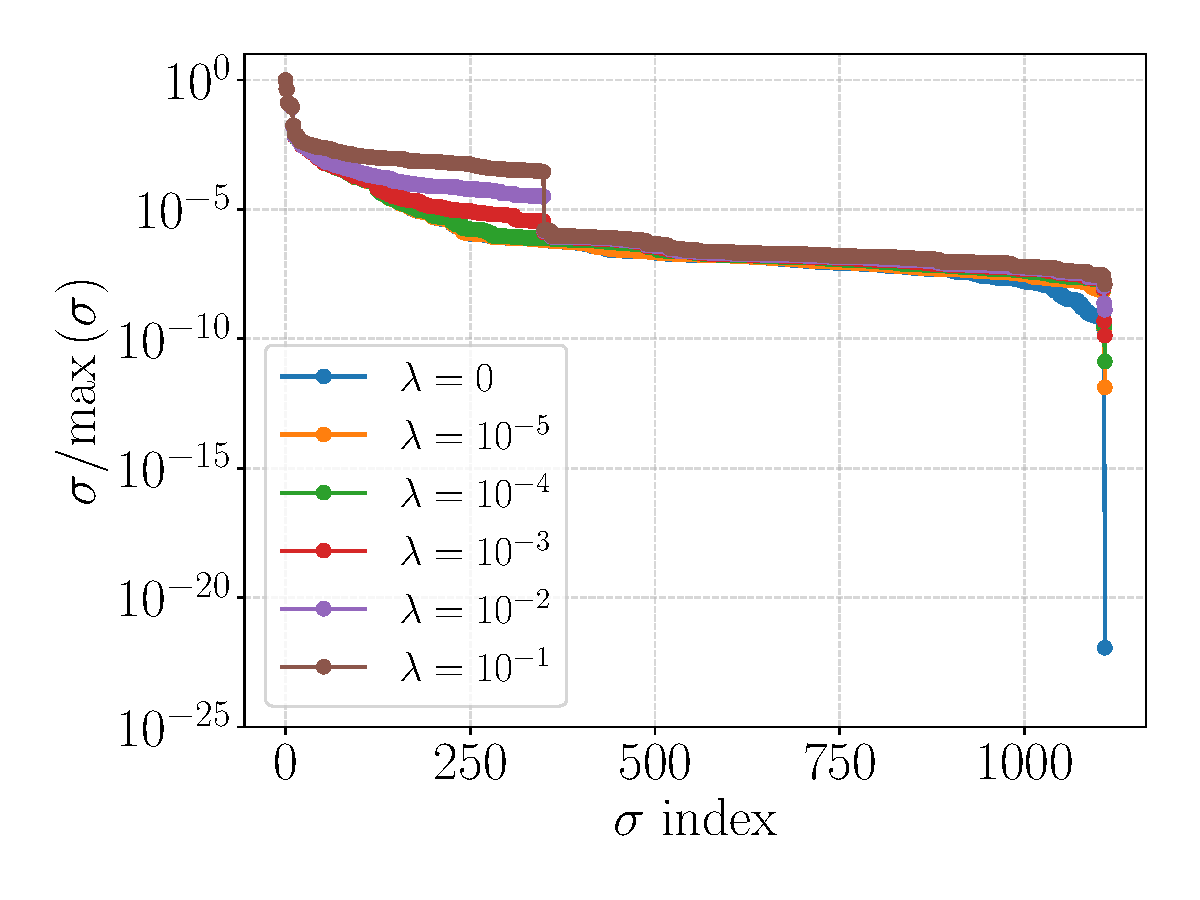
\includegraphics[width=1.0\textwidth]{figures/lm_singular_values_big_new.pdf}
    \caption{Levenberg-Marquardt.}
    \label{subfig:lm}
\end{subfigure}
 \begin{subfigure}[t]{0.49\textwidth}
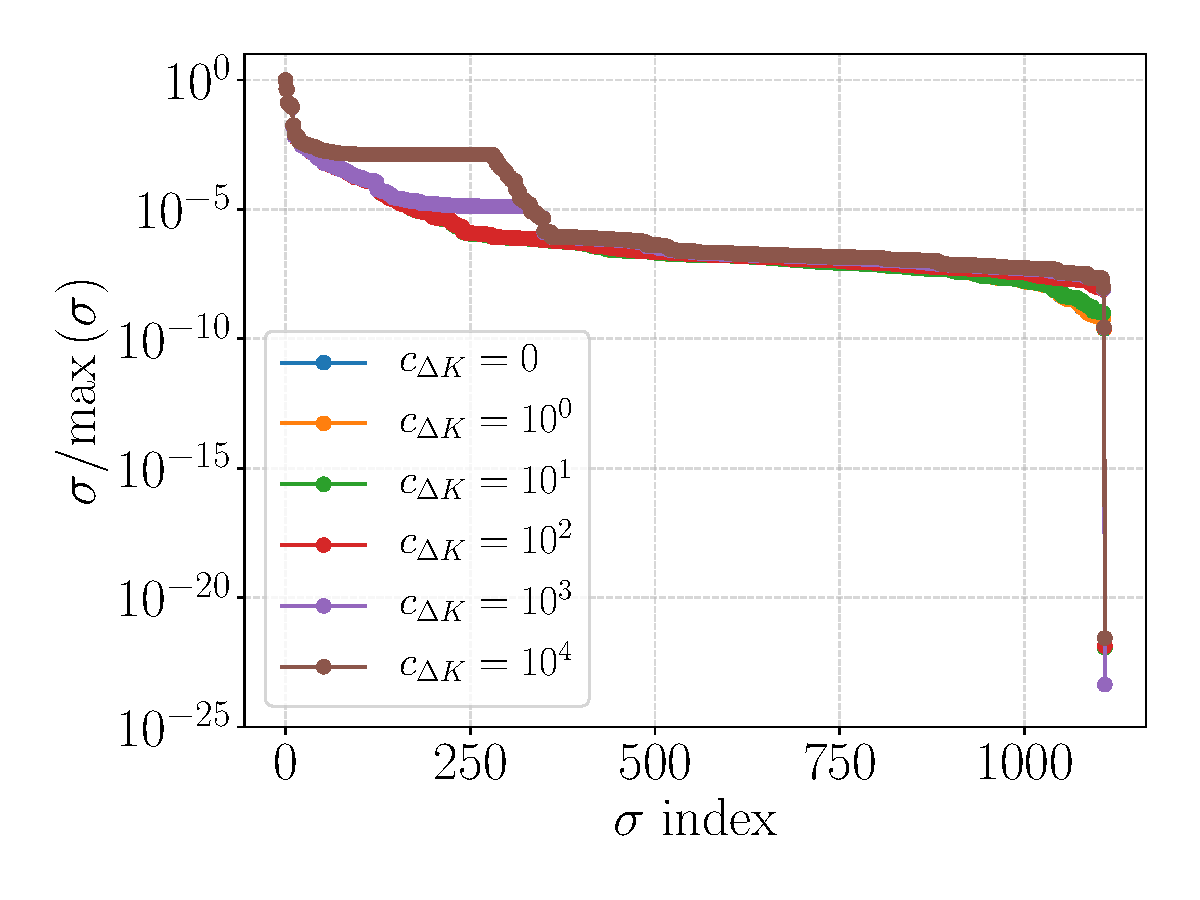
\includegraphics[width=1.0\textwidth]{figures/constraint_singular_values_big_new.pdf}
    \caption{$\Delta K$ constraint, $c_{\Delta K} = w_{\Delta K}/\sigma_{\Delta K}$.}
    \label{subfig:constraint}
\end{subfigure}
\caption{Effect of LM method and $\Delta K$ constraint on singular values of LOCO jacobian matrix.}
\label{fig:singval}
\end{figure}

The jacobian matrix in this analysis includes the~\gls{rf} response elements, i.e., the horizontal dispersion function is included, so the very low singular value $\sim10^{-21}$ for $\lambda = 0$ is related to the degeneracy between the vertical BPMs and correctors gains. With $\lambda = 10^{-5}$ this low singular value is already increased to $\sim10^{-12}$ and the decreasing singular values around $10^{-9}$ in the blue line are also raised. 
% Increasing the value of $\lambda$ introduces a clear step at the $350\ts{th}$ singular value, which is related to the magnet's strengths parameters: $270$ normal quadrupoles plus $80$ skew quadrupoles. The remaining $760$ singular values are related to the BPMs and correctors parameters and their magnitude decreases very slowly. The first $12$ singular values stand out with relative strengths greater than $10^{-2}$ compared to the maximum. These values are related to the $12$ quadrupoles families and since these families are directly related to the lattice periodicity, the first $12$ singular values reflects the importance of the signature of symmetric gradient changes in the~\gls{orm}. 

In the literature~\cite{icfa_huang, huang2013}, it is recommended to start the fitting with $\lambda = 10^{-3}$. From Figure~\ref{subfig:lm} it can be seen that this value raises the singular value at the low end. Increasing $\lambda$ even further raises most of the singular values. Therefore using $\lambda=10^{-3}$ should prevent the problems related to the low singular values while greater values for $\lambda$ produce changes in the singular values that may slow the solution convergence.

Figure~\ref{subfig:constraint} shows the singular values for several constraint magnitudes. The weight vector was set as unity for every element and the normalization constant $\sigma_{\Delta K}$ was changed from $0$ to $10^{-4}$. The case $c_{\Delta K} = 0$ coincide with $\lambda = 0$ in the Figure~\ref{subfig:lm}. The normalization $\sigma_{\Delta K}$ can be interpreted as the limit of step variation in $\Delta K$. The typical values for the quadrupole gradients in Sirius storage ring are on the order of $10^{-2}$. Then setting the constraint on step size to $\Delta K \sim 10^{-2}$ does not really limits the gradients variations and this can be seen in the similar singular values distributions for $c_{\Delta K}$ from $0$ to $10^{2}$. Only with $c_{\Delta K}=10^{3}$ the changes in singular values are substantial. Notice that some singular values at low end are also raised with the $\Delta K$ constraints, these low singular values are related to the quasi-degeneracies between quadrupoles that may lead to large excursions in quadrupole gradients when no constraints are used.

Limiting too much the $\Delta K$ step variation may increase unnecessarily the number of iterations required for LOCO convergence. Hence, in the literature~\cite{icfa_huang, huang2013} it is recommended to use the maximum value of $\sigma_{\Delta K}$ that still produces a significant change in the singular values, aiming to balance the $\Delta K$ constraints and the number of iterations, therefore reducing LOCO running time whenever it is worth it. For Sirius storage ring, the optimum value was determined to be $\sigma_{\Delta K} = 10^{-3}$, thus $c_{\Delta K} = 10^{3}$.

Notice that with $c_{\Delta K}=10^{3}$ the last singular value was relatively smaller compared to the unconstrained case. This can be solved by combining the constrained case with the~\gls{lm} minimization, given that it was seen that the~\gls{lm} contribution raises the singular values. The singular values distribution for the chosen values of $\lambda$ and $c_{\Delta K}$ compared to the original distribution are shown in Figure~\ref{fig:compare_svs}. The last singular value is associated with the gain degeneracy between vertical~\glspl{bpm} and correctors, so, in principle, it is the only singular value that should be removed.
\begin{figure}
\centering
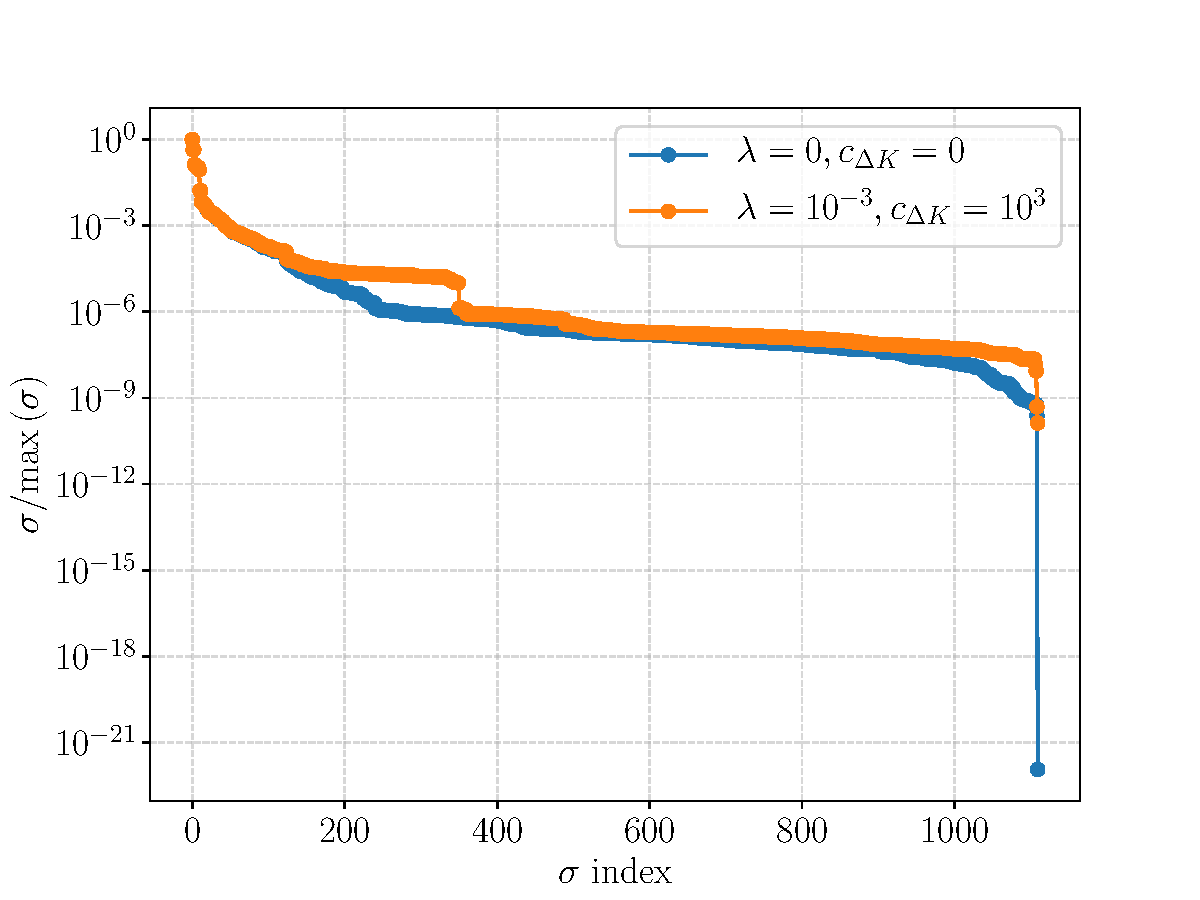
\includegraphics[width=0.70\textwidth]{figures/chosen_singular_values.pdf}
\caption{Singular values distributions between GN unconstrained method and LM constrained method with chosen parameters.}
\label{fig:compare_svs}
\end{figure}